% -*- mode: latex; -*-
\documentclass{beamer}

\usepackage{graphicx}
\usepackage{tikz}
\usetikzlibrary{shapes,calc,arrows,chains,decorations.pathmorphing,backgrounds,positioning,fit,scopes}

\usepackage{listings}

\setbeamersize{text margin left = 0.2em}
\setbeamersize{text margin right = 0.2em}

\title{A REST API for the groupware Kolab with support for different Media Types}
\subtitle{Bachelor Thesis}
\date{\today}
\author{Thomas Koch}


\newcommand{\entry}[1]{\node[entry, on chain]{entry \emph{#1}};}
\newcommand{\deleted}[1]{\node[deleted, on chain]{deleted \emph{#1}};}
\newenvironment{feed}[1]
  {\begin{scope} [start chain=#1,%
                  node distance=0.4ex%
                 ]%
  }
  {\end{scope}}
\newcommand{\feedsbackgrounds}[1]{%
  \begin{pgfonlayer}{background}%
    \foreach \x in {#1} {%
      \node[fit=(\x-begin) (\x-end),feedbackground] (\x-background) {};%
    }%
  \end{pgfonlayer}%
}
\newcommand{\metatext}{\emph{meta:} title, id, author, updated}
\newcommand{\nextlinktext}{\emph{link:} next feed}
\newcommand{\meta}{\node[meta, on chain] {\metatext \\ \nextlinktext };}
\newcommand{\metalast}{\node[meta, on chain] {\metatext \\ (no next link)};}
\newcommand{\nextlink}[2]{%
  \draw[ultra thick,->] (node cs:name=#1-begin,angle=342)%
     to [out=0,in=225] ($(node cs:name=#1-background,anchor=north)!.55!(node cs:name=#2-background,anchor=north)+(0,1em)$)%
     to [out=45,in=90] (node cs:name=#2-background,anchor=north);%
}

\newcommand{\feedspicture}[3]{%
\begin{tikzpicture}[feedspicture]%
  \matrix [feedsmatrix] {%
    \begin{feed}{feeda}%
      \meta #1%
    \end{feed} \pgfmatrixnextcell  %
    \begin{feed}{feedb}%
      \meta #2 %
    \end{feed}   \pgfmatrixnextcell %
    \begin{feed}{feedc}%
      \metalast #3%
    \end{feed} \pgfmatrixendrow %
  };%
%
  \feedsbackgrounds{feeda,feedb,feedc}%
  \nextlink{feeda}{feedb}%
  \nextlink{feedb}{feedc}%
\end{tikzpicture}%
}

\newcommand{\img}[1]{ \includegraphics[width=\textwidth]{images/#1.png} }
\newcommand{\imgopt}[2]{ \includegraphics[#1]{images/#2.png} }

\tikzset{feedspicture/.style={chain default direction=going below},
     feedbackground/.style={fill=orange!100,draw=black!100,inner xsep=0},
     feedelement/.style={
       minimum size=2em,
       minimum width=8em,
       rectangle,
       very thin
     },
     meta/.estyle={feedelement},
     meta/.append style={
       text width=8em,
       align=left,
       outer sep=0
     },
     entry/.estyle={feedelement},
     entry/.append style={
       draw=gray!100,
       fill=lightgray!30,
       font=\itshape
     },
     deleted/.estyle={feedelement},
     deleted/.append style={
       dashed,
       draw=gray!100,
       fill=lightgray!30!red!70,
       font=\itshape
     },
     feedsmatrix/.style={column sep=1.5em}
}

\begin{document}

\maketitle

\begin{frame}
  \tableofcontents
\end{frame}
\section{Kolab}

\begin{frame}{Kolab}
  \begin{itemize}
  \item started 2002
  \item free MS Exchange replacement for German BSI
  \item contacts, calendar, notes, tasks, journals
  \item IMAP server as storage and synchronization protocol
  \end{itemize}
\end{frame}

\begin{frame}{Kolab architecture}
  \begin{tikzpicture}[]
    { [every node/.style={text width=10em, node distance=10em}]
      \node (postfix) [label={SMTP}] { \img{postfix} };
      \node (cyrus) [below of=postfix,label={IMAP}] { \img{cyrus} };
      \node (apache) [right of=postfix,label={Web Interface}, node distance=20em] { \img{apache-php} \\ Apache+PHP mit \\ Horde/Roundcube };
      \node (openldap) [below of=apache,label={Verzeichnisdienst}] { \img{openldap} };
    }
    { [every edge/.style={draw,ultra thick}]
    \node [align=left, draw, dashed, inner sep=0.5ex]
       at ($(cyrus)!.5!(apache)$) {Kolab daemon,\\Scripts:\\Perl, Python}
       edge[->] (postfix)
       edge[->] (cyrus)
       edge[->] (apache)
       edge[<-] (openldap);
    }
  \end{tikzpicture}
\end{frame}

\begin{frame}{Clients need Kolab specific connectors}
  \begin{center}
  \begin{tikzpicture}
    { [node distance=13em, every edge/.style={draw,ultra thick}]
     \node [text width=15em, align=center, draw, dotted] (cyrus) {\imgopt{width=7em}{cyrus} \\ IMAP folders for \\ contacts, calendar, notes, \ldots};
     \node [below left of=cyrus,label={below:Gnome Evolution}] { \imgopt{width=7em}{evolution}}
       edge[<->] (cyrus) ;
     \node [below of=cyrus,label={below:KDE Kontact}] { \imgopt{width=7em}{kontact}}
       edge[<->] (cyrus) ;
     \node [below right of=cyrus,label={below:Mozilla Thunderbird}] { \imgopt{width=7em}{thunderbird}}
       edge[<->] (cyrus) ;

    }
  \end{tikzpicture}
  \end{center}
\end{frame}

\section{media types}
\begin{frame}{support for different client types}
  \begin{itemize}
  \item desktop apps \tt{$\rightarrow$ vCard (IMF) / xCard (XML)}
  \item browsers \tt{$\rightarrow$ (X)HTML + semantic annotation}
  \item js widgets \tt{$\rightarrow$ PortableContacts (JSON)}
  \end{itemize}
\end{frame}

\begin{frame}{media type conversion and non-isomorphism}

  \begin{tabular}{p{20em} p{10em}}
approaches:
 \begin{itemize}
  \item only one media type for writes
  \item special PATCH media types
  \item restrict types to common denominator
  \item extend media types to reach isomorphism
  \item ignore the problem, maybe do version control
 \end{itemize} &
   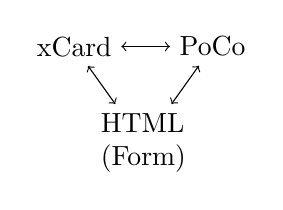
\begin{tikzpicture}
     \node (xcard) {xCard};
     \node (poco) at (5em,0) {PoCo}
       edge[<->] (xcard);
     \node [align=left] (html) at (2.5em,-3.5em) {HTML\\(Form)}
       edge[<->] (xcard)
       edge[<->] (poco);
   \end{tikzpicture}
  \end{tabular}
\end{frame}

\section{interactions}

\begin{frame}{Atom Publishing Protocol, hypermedia}
  \begin{center}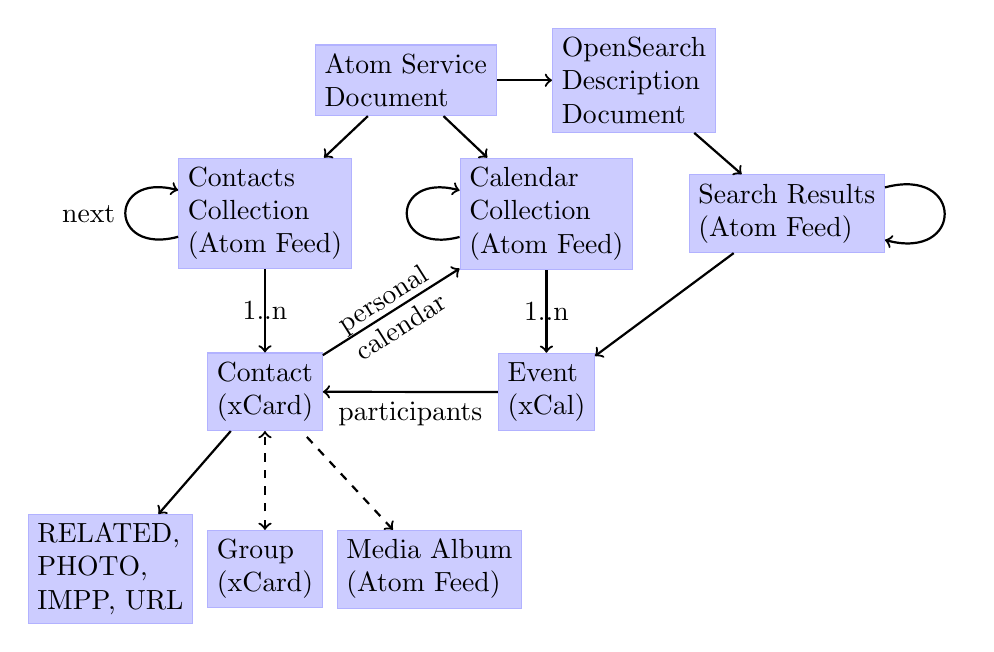
\begin{tikzpicture}[
    align=left,
    every loop/.style={looseness=4},
    every edge/.style={draw, thick},
    doc/.style={rectangle,
                draw=blue!30,fill=blue!20,
                node distance=3em and 0.5em}]
    \node[doc] (svc) [] {Atom Service\\Document};
    \node[doc] (collect) [below left=1.5em and 1.8em of svc,anchor=north] {Contacts\\Collection\\(Atom Feed)}
      edge [<-] node {} (svc)
      edge [->, loop left] node {next} (collect);

    \node[doc] (calcollect) [below right=1.5em and 1.8em of svc,anchor=north] {Calendar\\Collection\\(Atom Feed)}
      edge [<-] node {} (svc)
      edge [->, loop left] node [] {} (calcollect);

    \node[doc] (opensearch) [right=2em of svc] {OpenSearch\\Description\\Document}
      edge [<-] node {} (svc);

    \node[doc] (entry) [below=of collect] {Contact\\(xCard)}
      edge [<-] node {1..n} (collect)
      edge [->] node [sloped] {personal\\calendar} (calcollect);

    \node[doc] (event) [below=of calcollect] {Event\\(xCal)}
      edge [<-] node {1..n} (calcollect)
      edge [->] node [below] {participants} (entry);

    \node[doc] (searchresult) [right=2em of calcollect] {Search Results\\(Atom Feed)}
      edge [->] node {} (event)
      edge [->, loop right] node [] {} (searchresult)
      edge [<-] node {} (opensearch);

    \node[doc] (social) [below left=of entry] {RELATED,\\PHOTO,\\IMPP, URL}
      edge [<-] node {} (entry);

    \node[doc] (group) [right=of social] {Group\\(xCard)}
      edge [<->,style=dashed] node {} (entry);

    \node[doc] (album) [right=of group] {Media Album\\(Atom Feed)}
      edge [<-,style=dashed] node {} (entry);
  \end{tikzpicture}\end{center}
\end{frame}

\begin{frame}[t]{feed after 11 POSTs}
\feedspicture
{ \entry{11} \entry{10} \entry{9} \entry{8} }
{ \entry{7}  \entry{6}  \entry{5} \entry{4} }
{ \entry{3}  \entry{2}  \entry{1} }
\url{http://myapi.org/.../contacts?offset=0|4|8}
\\
feed entries link to full representations
\\
feed entries sorted by edited time
\end{frame}

\begin{frame}[t]{POST new entry to feed}
\feedspicture
{ \entry{12} \entry{11} \entry{10} \entry{9} }
{ \entry{8}  \entry{7}  \entry{6}  \entry{5} }
{ \entry{4}  \entry{3}  \entry{2}  \entry{1} }
\end{frame}

\begin{frame}[t]{PUT updated entry 6}
\feedspicture
{ \entry{6} \entry{12} \entry{11} \entry{10} }
{ \entry{9} \entry{8}  \entry{7}  \entry{5} }
{ \entry{4} \entry{3}  \entry{2}  \entry{1} }
\end{frame}

\begin{frame}[t]{DELETE entry 2}
\feedspicture
{ \deleted{2}  \entry{6}  \entry{12} \entry{11} }
{ \entry{10} \entry{9}  \entry{8}  \entry{7} }
{ \entry{5}  \entry{4}  \entry{3}  \entry{1} }
\end{frame}

\begin{frame}[t]{Many more changes}
\feedspicture
{ \entry{7}  \entry{4}  \entry{10} \deleted{11} }
{ \entry{8} \deleted{9}  \entry{1}  \entry{3} }
{ \entry{5}  \entry{12}  \deleted{2}  \entry{6} }
\end{frame}

\begin{frame}[t]{update of entry 6}
\feedspicture
{ \entry{6} \entry{7}  \entry{4}  \entry{10} }
{ \deleted{11} \entry{8} \deleted{9}  \entry{1} }
{ \entry{3} \entry{5}  \entry{12}  }
\end{frame}

\section{implementation}

\begin{frame}{Execution flow overview}
  \begin{center}
    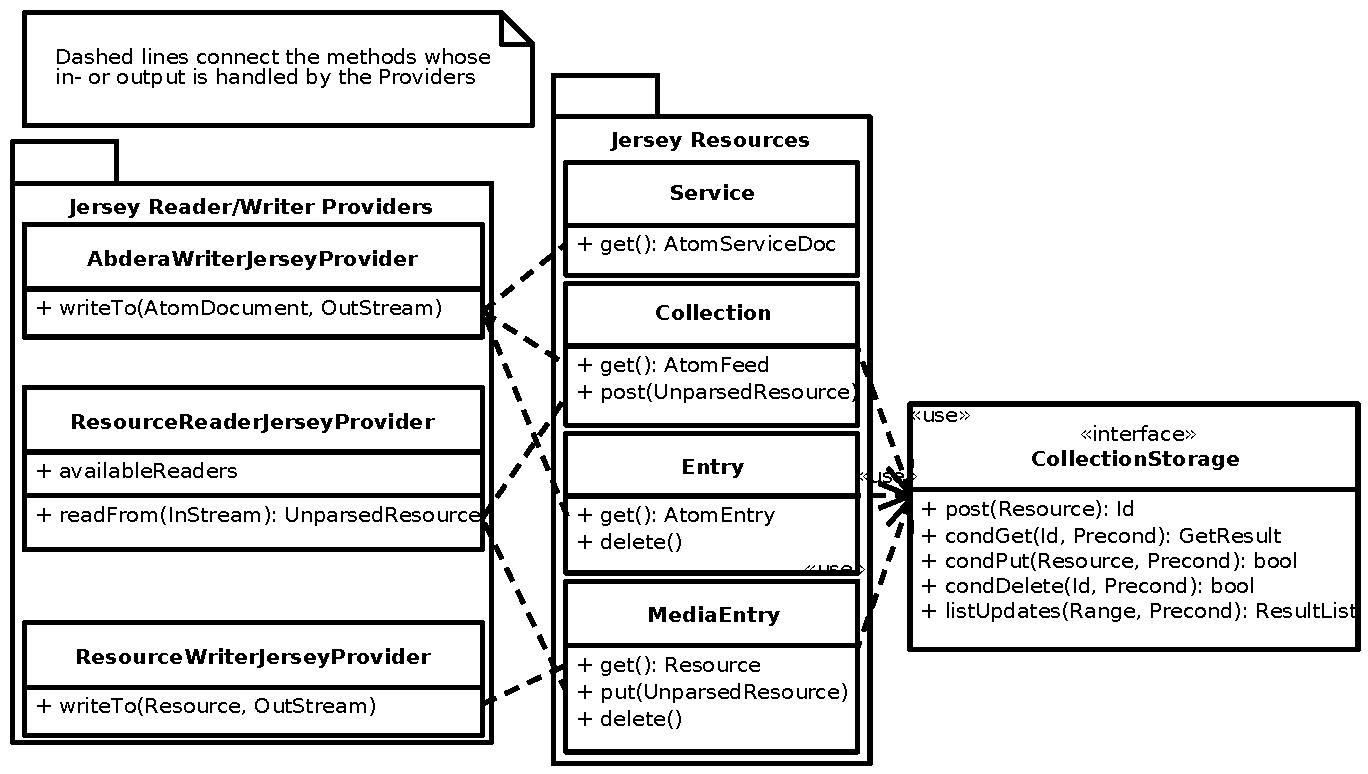
\includegraphics[width=1\textwidth]{images/executionflowoverview}
  \end{center}
\end{frame}

\begin{frame}{Resource Properties}
\begin{itemize}
\item essential administration properties: unique ID, last update time, HTTP
  entity tag
\item generic meta properties: title, summary, author
\item a media type independent interface corresponding to the concept represented
  by the resource, e.g., a person, location, event, product, \ldots
\item a media type specific serialization (representation) of the resource
\end{itemize}

\end{frame}

\begin{frame}{Facades and their dependencies}
  \begin{center}
    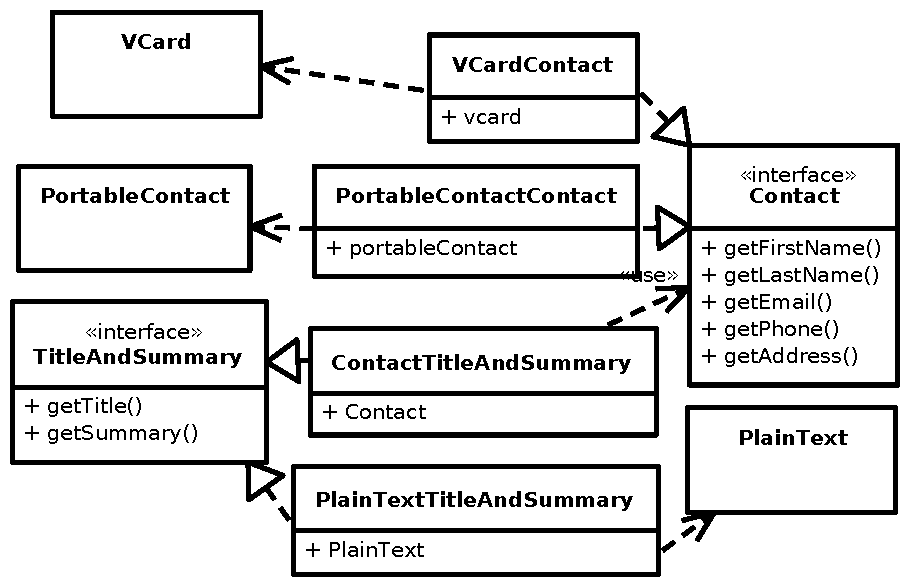
\includegraphics[width=1\textwidth]{images/titleandsummary}
  \end{center}
\end{frame}

\begin{frame}{Facades implementation}
  \begin{center}
    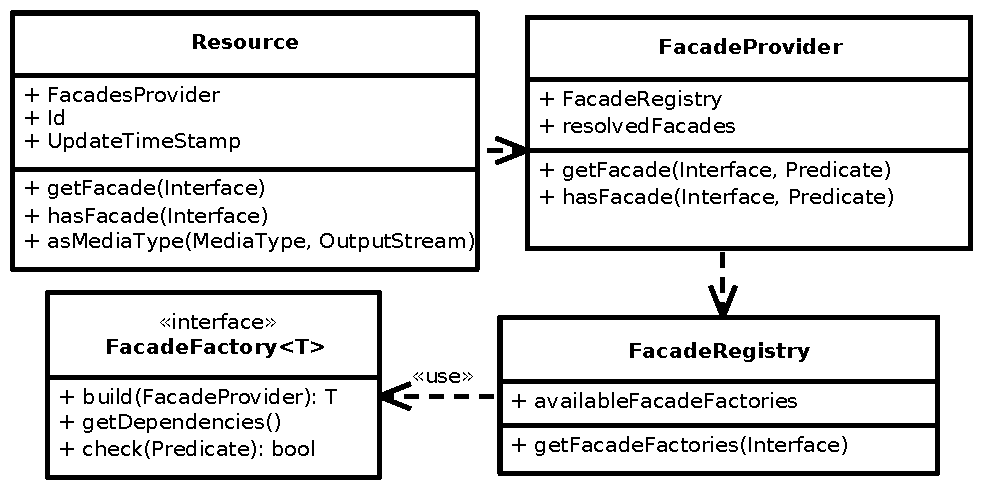
\includegraphics[width=1\textwidth]{images/resourcefacades}
  \end{center}
\end{frame}

\begin{frame}{Dependency Injection}
  \begin{center}  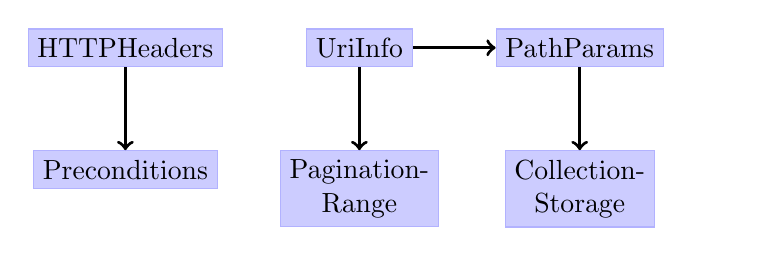
\begin{tikzpicture}[
     align=center,
     every edge/.style={draw,very thick},
     doc/.style={rectangle,draw=blue!30,fill=blue!20, node distance=3em}]

    \node[doc] (uriinfo) [] {UriInfo};

    \node[doc] (httpheaders) [left=of uriinfo] {HTTPHeaders};

    \node[doc] (Preconditions) [below=of httpheaders] {Preconditions}
      edge [<-] node [] {} (httpheaders);

    \node[doc] (PaginationRange) [below=of uriinfo] {Pagination-\\Range}
      edge [<-] node [left] {} (uriinfo);

    \node[doc] (pathparams) [right=of uriinfo] {PathParams}
      edge [<-] node [above] {} (uriinfo);

    \node[doc] (collection) [below=of pathparams] {Collection-\\Storage}
      edge [<-] node [right,text width=5em] {} (pathparams);

  % \begin{pgfonlayer}{background}
  %     \node[fit=(httpheaders) (collection),draw, dashed,fill=lightgray!50, inner sep=1em] () {};
  % \end{pgfonlayer}

  \end{tikzpicture} \end{center}
\end{frame}

\begin{frame}{isolate URI handling}
  \begin{itemize}
  \item processing: PaginationRange, PathParam, Router class
  \item construction: LinkBuilder
  \item URI details are classified information $\rightarrow$ enforce hypermedia
  \end{itemize}
  no \lstinline:@Path:, \lstinline:@PathParam:, \lstinline:@QueryParam: annotations!
\end{frame}

\section{problems, findings, future work}

\begin{frame}{problems: media type libraries}
  \begin{itemize}
    \item only vCard 3, no vCard / xCard 4
    \item 2 dead PortableContact libraries
    \item no existing conversion code
    \item no helper for semantic annotation
  \end{itemize}
  \pause
  \ldots but dozens of HTTP libraries
\end{frame}

\begin{frame}[fragile]{Semantic annotation helper}
\lstset{frame=single,
        backgroundcolor=\color{lightgray!50}
}
  \begin{lstlisting}
div( itemscope itemtype="http://schema.org/Person"
     itemid=#{vcard.getProperty("uid")} )
  span( itemprop="name" )
    #{vcard.getProperty("fn")}
  span( itemprop="telephone" )
    #{vcard.getProperty("tel")}
  \end{lstlisting}
let md be a MicroData aware helper object:
  \begin{lstlisting}
= md.scope
  div
    = md.prop("name")
      span( style="color:red" )
    = md.prop("telephone")
    = md.prop("email")
  \end{lstlisting}
\end{frame}

\begin{frame}{Kolab}
  \begin{itemize}
  \item ANNOTATEMORE (draft) $\rightarrow$ METADATA (RFC 5464) $\rightarrow$ Special-Use Mailboxes (RFC 6154)
  \item vCard 3 $\rightarrow$ Kolab XML $\rightarrow$ xCard 4
  \item documented by code
  \item works only with Cyrus, not with Dovecot
  \end{itemize}
\end{frame}

\begin{frame}
  \begin{itemize}
  \item concentration on media types
  \item JAX-RS not helpful
  \item ATOM is versatile
  \end{itemize}
\end{frame}

\end{document}
